% Template for Cogsci submission with R Markdown

% Stuff changed from original Markdown PLOS Template
\documentclass[10pt, letterpaper]{article}

\usepackage{cogsci}
\usepackage{pslatex}
\usepackage{float}
\usepackage{caption}

% amsmath package, useful for mathematical formulas
\usepackage{amsmath}

% amssymb package, useful for mathematical symbols
\usepackage{amssymb}

% hyperref package, useful for hyperlinks
\usepackage{hyperref}

% graphicx package, useful for including eps and pdf graphics
% include graphics with the command \includegraphics
\usepackage{graphicx}

% Sweave(-like)
\usepackage{fancyvrb}
\DefineVerbatimEnvironment{Sinput}{Verbatim}{fontshape=sl}
\DefineVerbatimEnvironment{Soutput}{Verbatim}{}
\DefineVerbatimEnvironment{Scode}{Verbatim}{fontshape=sl}
\newenvironment{Schunk}{}{}
\DefineVerbatimEnvironment{Code}{Verbatim}{}
\DefineVerbatimEnvironment{CodeInput}{Verbatim}{fontshape=sl}
\DefineVerbatimEnvironment{CodeOutput}{Verbatim}{}
\newenvironment{CodeChunk}{}{}

% cite package, to clean up citations in the main text. Do not remove.
\usepackage{apacite}

% KM added 1/4/18 to allow control of blind submission
\cogscifinalcopy

\usepackage{color}

% Use doublespacing - comment out for single spacing
%\usepackage{setspace}
%\doublespacing


% % Text layout
% \topmargin 0.0cm
% \oddsidemargin 0.5cm
% \evensidemargin 0.5cm
% \textwidth 16cm
% \textheight 21cm

\title{Predicting graded dishabituation using perceptual stimulus
embeddings in a rational learning model}


\author{ Anjie Cao*$^1$ (anjiecao@stanford.edu), Gal Raz*$^2$ (galraz@mit.edu)\\, \bf{Rebecca Saxe$^2$ (saxe@mit.edu)},
 and  \bf{Michael C. Frank$^1$ (mcfrank@stanford.edu)}, \\
$^1$Department of Brain and Cognitive Sciences, MIT, $^2$Department of Psychology, Stanford University \\ }

\newlength{\cslhangindent}
\setlength{\cslhangindent}{1.5em}
\newenvironment{CSLReferences}%
  {}%
  {\par}

\begin{document}

\maketitle

\begin{abstract}
How do humans decide what to look at and when to stop looking? The
Rational Action, Noisy Choice for Habituation (RANCH) model formulates
looking behaviors as a rational information acquisition process. RANCH
instantiates a hypothesis about the perceptual encoding process using a
neural network-derived embedding space, which allows it to operate on
raw images. In this paper, we show that the model not only captures key
looking time patterns such as habituation and dishabituation, but also
makes fine-grained, out-of-sample predictions about magnitudes of
dishabituation to previously unseen stimuli. We validated those
predictions experimentally with a self-paced looking time task in adults
(N = 468). We also show that model fits are robust across parameters,
but that assumptions about the perceptual encoding process, the learning
process and the decision process are all critical for predicting human
performance.

\textbf{Keywords:}
attention; learning; visual perception; bayesian models
\end{abstract}

\hypertarget{introduction}{%
\section{Introduction}\label{introduction}}

From birth, humans learn actively. Even before they can move on their
own, infants can select information by deciding what to look at and when
to stop looking (Haith, 1980; Raz \& Saxe, 2020). Developmental
psychologists have long leveraged this attentional decision-making to
make inferences about the perceptual and cognitive abilities of infants
by measuring how long infants look at certain stimuli (Aslin, 2007;
Baillargeon, Spelke, \& Wasserman, 1985; Fantz, 1963).

Two key phenomena are particularly critical for these inferences:
habituation and dishabituation. Habituation refers to the decrease in
looking time upon seeing the same or similar stimuli repeatedly;
dishabituation refers to the increase in looking time following the
presentation of a novel stimulus after habituation. In order to
dishabituate, the infant must distinguish between the original stimulus
and the novel one. While habituation and dishabituation have been
robustly documented, the underlying mechanisms of these looking time
changes remain poorly understood. In this paper, we address this gap by
presenting a rational model that provides principled predictions about
the magnitude of dishabituation. Critically, this model can be applied
generally to make predictions about looking time for arbitrary stimuli
by using embeddings derived from a convolutional neural network.

The dominant model of infant looking time proposes that habituation and
dishabituation are driven by the amount of information to be encoded in
the stimulus (Hunter \& Ames, 1988). Observers look longer at a stimulus
if the stimulus has a lot of unencoded information, and as exposure to
the stimulus accumulates, less information is left unencoded, leading to
shorter looking time. While this theory has been highly influential, the
lack of formal details about what is meant by ``encoding'' opens the
door for post-hoc interpretation of looking time measurements. A
stimulus could be argued to be novel because it has distinct perceptual
features, but it could also be familiar because of its conceptual
characteristics (or perhaps both at the same time). In part as a result
of this interpretive ambiguity, concerns have been raised repeatedly
about whether looking time measurements should be the foundation for
central claims in developmental psychology (Blumberg \& Adolph, 2023;
Haith, 1998; Paulus, 2022).

Computational models provide an important tool for formalizing the
details of the habituation and dishabituation process. One set of models
describes infants' looking behaviors with information-theoretic measures
derived from ideal observer models (Kidd, Piantadosi, \& Aslin, 2012;
Francesco Poli, Ghilardi, Mars, Hinne, \& Hunnius, 2023; F. Poli,
Serino, Mars, \& Hunnius, 2020). For example, Poli et al.~(2023)
developed a model that learned probability distributions from sequences
of events. They then calculated the Kullback--Leibler (KL) divergence
between the model's parameters before and after each event in a
sequence, capturing how much the model learned from each observation.
This measure was shown to predict infants' looking behavior, with higher
KL associated with lower probabilities of infants looking away.

While this type of model provides a quantitative account of the
habituation process, it does not model the infant's information sampling
process directly. Instead, it describes trial-level correlations between
model-derived, information-theoretic measures and infant looking times.
Essentially, this type of model fails to elucidate the causal
relationship between information theoretic measurements and infant's
samling decision. Furthermore, it presupposes an abstracted
representation of the stimuli as a sequence of schematic events (e.g.,
1, 2, 1, 1, 3, etc.) rather than instantiating a hypothesis about how
visual encoding occurs during attentional decision-making. This feature
limits the ability of these models to make principled predictions about
looking time for new stimuli.

To address these issues, Rational Action, Noisy Choice for Habituation
(RANCH) model was developed (Cao, Raz, Saxe, \& Frank, 2023; Raz, Cao,
Saxe, \& Frank, 2023). RANCH describes an agent's looking behavior as
rational exploration based on a sequence of noisy perceptual samples.
The model construes the looking time paradigm as a series of binary
decisions: to keep sampling from the current stimulus, or to move on to
the next stimulus. The model makes sampling decisions based on the
Expected Information Gain (EIG) of the perceptual samples, choosing to
keep looking or look away based on which one would in expectation yield
the most information; it therefore can be seen as a rational analysis of
looking behavior (Anderson, 1991; Lieder \& Griffiths, 2020; Oaksford \&
Chater, 1994).

RANCH also incorporates recent progress in convolutional neural
networks, which have offered insights into how the visual system encodes
objects (Doshi \& Konkle, 2023; Hebart, Zheng, Pereira, \& Baker, 2020;
Yamins et al., 2014). The activations of these brain-inspired neural
networks form embedding spaces, each of which can be seen as a
quantitative hypothesis about how humans represent visual stimuli
(Schrimpf et al., 2020). For example, Lee (2022) projected the final
layer of a trained ResNet50 into a ``perceptually-aligned'' space, by
making its representations match dissimilarity matrices derived from
human adult reaction times in a 2-AFC match-to-sample task. Passing new
stimuli through this perceptual alignment yields a plausible
representation of how humans embed different visual stimuli in a
low-dimensional space. Using this perceptually-aligned embedding space
as a model of perceptual encoding allows RANCH to learn from raw,
previously unseen images.

Previously, Cao et al. (2023) and Raz et al. (2023) have shown that
RANCH can successfully model habituation and dishabituation in adults
and infants. In this paper, we test RANCH's ability to predict responses
in new data, particularly a key phenomenon in qualitative accounts of
dishabituation. To conduct these tests, we first fit RANCH's parameters
to a training dataset from the habituation-dishabituation experiment in
which participants saw sequences of monsters which were either familiar
or novel (dataset reported in Cao et al., 2023, Fig 1A). Then, we use
the best-fitting parameters to generate predictions for a new experiment
designed to measure subtle differences in dishabituation magnitude based
on stimulus similarity (Fig 1C). In this new experiment, we
systematically varied the similarity between habituation and
dishabituation stimuli such that dishabituation stimuli differed in
their pose angle, their number, their identity, or their animacy. This
experiment tests a prediction from Hunter \& Ames (1988) model of
habituation and dishabituation: that observers' dishabituation magnitude
should be related to the similarity between the habituated stimulus and
the novel stimulus. The more dissimilar two stimuli are, the more one
should dishabituate to the novel stimulus.

To preview our results, we show that RANCH can predict looking time
responses in new data by transferring model parameters fit from previous
data, with marginal differences in performance compared to completely
refitting to the new data. RANCH also captures the particular ordering
of the dishabituation magnitude as a function of stimulus dissimilarity,
thereby predicting a novel qualitative phenomenon (graded
dishabituation) without ever being trained on it. Finally, we show that
RANCH is relatively robust across parameter settings, but the
assumptions about its perceptual representation, learning process, and
the decision process are all critical to its performance.

\hypertarget{model}{%
\section{Model}\label{model}}

\begin{CodeChunk}
\begin{figure*}[h!]

{\centering 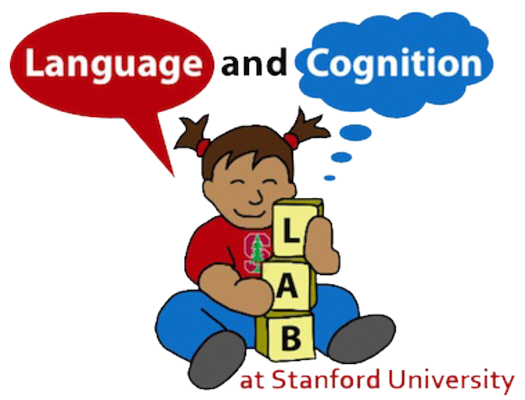
\includegraphics{figs/design_fig-1} 

}

\caption[Workflow of the current study]{Workflow of the current study. (A) The experimental design and stimuli used in the training dataset. (B) The core components of RANCH, with the top showing the stimuli embedding in PC-space. The bottom is the plate diagram of the learning model. (C) The experimental design of the test data. RANCH model is first fit using the training data in A, and we test its prediction on the test data collected in the experiment illustrated in C.}\label{fig:design_fig}
\end{figure*}
\end{CodeChunk}

\hypertarget{model-components}{%
\subsection{Model Components}\label{model-components}}

We modeled looking behaviors in our task as rational information
acquisition, using a rational analysis approach previously described for
different information-seeking behaviors (Dubey \& Griffiths, 2020;
Oaksford \& Chater, 1994). Our goal was to develop a model which
formalizes the entire process underlying looking time: from perception
of a stimulus to deciding how long to look at it. To do so, our model
has three separate components describing (1) how stimuli are embedded in
a low-dimensional perceptual space (2) how RANCH learns a concept over
this perceptual space and (3) how RANCH makes decisions about how long
to sample from a stimulus based on its expected information gain. Here,
we describe these three components in turn.

\hypertarget{perceptual-representation}{%
\subsubsection{Perceptual
representation}\label{perceptual-representation}}

To allow RANCH to operate on raw images, we used the
perceptually-aligned embeddings obtained from a model presented recently
by Lee (2022). We use these projections into a perceptually-aligned
embedding space as a principled low-dimensional representation of
stimuli, over which our learning model can form perceptual concepts. We
used the first three principal components of the embedding space due to
limits on the computing power; increasing dimension would lead to
exponential increase in the total run time. The first three components
captured 57.9\% of the variance. A visualization of experimental stimuli
in the embedding space can be seen in Figure 1B.

\hypertarget{learning-model}{%
\subsubsection{Learning model}\label{learning-model}}

RANCH's goal is to learn a concept in the perceptual embedding space
described above, through noisy perceptual samples from a stimulus. The
concept is parameterized by a single 3D Gaussian \((\mu,\sigma)\), which
represents beliefs about the location and variance of the concept in the
embedding space. This concept describes the distribution of all viewed
stimuli in this experiment. This concept \((\mu,\sigma)\) generates
exemplars \((y)\) of the concept. Each exemplar corresponds to one
stimulus observed. RANCH observes repeated noisy samples \((\bar{z})\)
from each exemplar. For any sample \((z)\) from an exemplar \((y)\), the
model expects the observation to get corrupted by zero-mean gaussian
noise with standard deviation \((\epsilon)\). A plate diagram is shown
in Figure 1B. We used a normal-inverse-gamma prior on the concept, the
conjugate prior for a normal with unknown mean and variance, on the
concept parameterized as \(\mu_{p}\),\(\nu_{p}\),\(\alpha_{p}\),
\(\beta_{p}\). Still, applying perceptual noise to \(y\) breaks the
conjugate relation, so we computed approximate posteriors using grid
approximation over \((\mu,\sigma)\) and \((\epsilon)\). This
computationally expensive approximation was accomplished through a
PyTorch implementation and distributed GPU computation.

\hypertarget{decision-model}{%
\subsubsection{Decision model}\label{decision-model}}

To decide whether to take an additional sample from the same stimulus,
RANCH computes Expected Information Gain (EIG) of the next sample. EIG
is computed as the product of the posterior predictive probability of
the next sample and the information gained conditioned on that next
sample, by iterating through a grid of possible subsequent samples.
RANCH then makes a softmax choice (with temperature = 1) between taking
another sample and looking away. We assumed that participants expect a
constant information gain from looking away (the ``world EIG'').
Therefore, as EIG from the stimulus drops below world EIG, it becomes
increasingly likely that RANCH will look away.

\hypertarget{alternative-models}{%
\subsection{Alternative models}\label{alternative-models}}

To test the importance of each of RANCH's components for its
performance, we defined three lesioned models, in which one key feature
of the model was removed in each model. First, to test the importance of
the perceptual embeddings, we ran a version of RANCH in which the
mappings from stimulus labels to embeddings were permuted, such that the
associations between embeddings and violation type were randomized
(``Random embeddings''). Second, we ran a version in which RANCH assumes
that each perceptual sample in the learning process is noiseless, rather
than corrupted by \(\epsilon\) (``No noise'').Third, we ran a version in
which RANCH made decisions randomly rather than based on the learning
model (``No learning'').

\hypertarget{training-procedure}{%
\subsection{Training Procedure}\label{training-procedure}}

We used the behavioral dataset reported in Cao et al. (2023) as the
training data. In this prior experiment, 449 adults participated in an
online self-paced looking time paradigm (Fig. 1A). In this paradigm,
participants watched blocks of six animated monsters. Each block
consisted of one repeating monster (the background), and one monster
different from the repeated one (the deviant). The deviant, if shown,
was on either the 2nd, 4th, or 6th trial of the block. Adults can
proceed to the next trial whenever they press a key on the keyboard, and
the interval between the onset of the stimuli and the key press was used
as the proxy for looking time. To train on this dataset, we first
converted the raw stimuli into perceptual embeddings, and combined them
into the same sequences the participants saw. Since the model makes
stochastic sampling decisions, we conducted 400 runs for each stimulus
sequence for each parameter setting. To avoid numerical instabilities
due to the granularity of our grid approximation, for each run we
slightly jittered all parameter grid values by a constant offset. We
conducted an iterative grid search across the priors over \(\mu\),
\(\nu\) and \(\epsilon\), along with the actual noise \(\epsilon\). We
selected the parameters that yielded the highest \(R^2\) between the
model output and the behavioral data as the best fitting parameters. The
best fitting parameters were: \(\mu_{p}\) = 0,\(\nu_{p}\) = 1,
\(\alpha_{p}\) = 1, \(\beta_{p}\) = 1, \(\epsilon\) = 0.0001.

\hypertarget{behavioral-experiment}{%
\section{Behavioral Experiment}\label{behavioral-experiment}}

Next, we introduce the novel experiment used to test the
generalizability of the parameter setting found above. The procedure was
similar to the previous training data with two key differences: First,
stimuli used in the training data were animated monsters, whereas the
current experiment (test data) used images of animals and vegetables
with added shaking animations. Second, unlike the training data, the
current experiment varied the dissimilarity between the repeating
stimuli and the deviant stimuli by introducing four different types of
deviant stimuli.

\begin{CodeChunk}
\begin{figure*}[h!]

{\centering 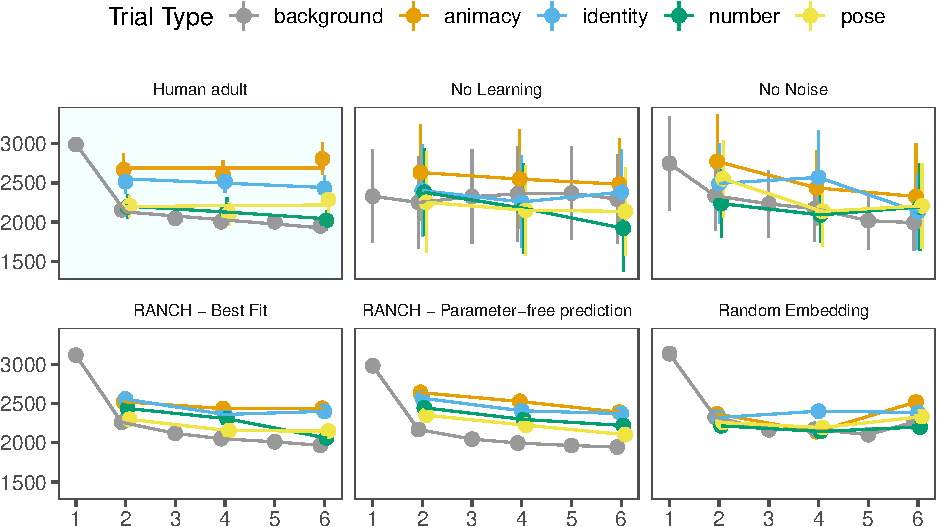
\includegraphics{figs/lol-1} 

}

\caption[RANCH and alternative models]{RANCH and alternative models. For the human panel, X-axis shows the trial number, y-axis shows the looking time at each trial to the test stimuli in milliseconds. The line shows the fit from the preregistered linear mixed effect model. For the remaining panels, Y-axis represents the samples model made on each trial, scaled linearly to the behavioral data. The scaling procedure was applied to each model individually. Different colors represent different trial types.}\label{fig:lol}
\end{figure*}
\end{CodeChunk}

\hypertarget{methods}{%
\subsection{Methods}\label{methods}}

\hypertarget{stimuli}{%
\subsubsection{Stimuli}\label{stimuli}}

All stimuli were created using images selected from Unity assets
\href{https://assetstore.unity.com/packages/3d/characters/animals/quirky-series-animals-mega-pack-vol-2-183280}{``Quirky
Series - Animals''} and
\href{https://assetstore.unity.com/packages/3d/props/food/3d-prop-vegetables-and-fruits-237790}{``3D
Prop Vegetables and Fruits''}. We added the same minor shaking animation
to each image to increase interest. For each image from the animal set,
we created a mirrored version to create an image with a different pose.
The long axis of each vegetable image was tilted before mirroring.

\hypertarget{procedure}{%
\subsubsection{Procedure}\label{procedure}}

The experiment was a self-paced web-based looking time experiment (Fig.
1C). Participants saw 24 blocks that consisted of either two, four, or
six trials. On each trial, a schematic screen would rise up to reveal a
stimulus behind it. Participants pressed the spacebar to go on to the
next trial after a minimum viewing time of 500 ms, triggering the
schematic screen to drop and raise again to reveal the next stimulus.

Each participant saw eight types of repeating stimuli. The eight types
of stimuli included all combinations of the three features that each
included two levels: animacy (e.g.~animals or vegetables), number
(singleton or pair), and pose (facing left or right).

Eight blocks consisted of one stimulus being repeatedly presented
throughout the block (background blocks). The remaining sixteen blocks
included two stimuli, including one that was repeatedly presented and
one that deviated from the repeating trial. Stimuli for each block were
randomly sampled from the stimulus pool without replacement. The deviant
trial was always different from the repeating stimulus in one of the
four dimensions: animacy, identity, number, and pose. The deviant trial
always appeared in the last trial of the block. In the first three
violation types, the feature would be switched to the previously unseen
level (e.g.~an inanimate deviant after an animate repeating stimulus,
keeping the number and the pose the same). For identity violations, the
participants would see a different, but within-category, exemplar from
the repeating stimulus category. Among the sixteen blocks, the four
violation types each appeared four times. After each block, participants
performed a filler task in which they judged whether they had seen an
animation before. Half of the filler task showed previously unseen
animation, and the other half showed an animation from the preceding
block.

To control the distribution of background blocks and deviant blocks, we
grouped the 24 blocks into four groups. Each group consisted of two
background blocks, and one deviant block from each violation type. The
order of blocks within each group was randomized.

\hypertarget{participants}{%
\subsubsection{Participants}\label{participants}}

We recruited 550 adult participants on Prolific. Participants were
excluded if either (1) the standard deviation of log-transformed of
their reaction times on all trials was less than 0.15 (indicating
key-smashing, e.g. Moon, 2021); (2) they spent more than three absolute
deviations above the median of the task completion time as reported by
Prolific, or (3) they provided the incorrect response to more than 20\%
of the memory task. In total, 15 \% of the participants were excluded by
these criteria. After the participant-level exclusion, we also applied
trial-level exclusion. A trial was excluded from final analysis if it
was three absolute deviations away from the median in the
log-transformed space across all participants. The final sample included
468 participants.

\hypertarget{results-and-discussion}{%
\subsection{Results and discussion}\label{results-and-discussion}}

The sample size and analysis plan were all pre-registered and can be
found \href{https://aspredicted.org/blind.php?x=WGF_J7K}{here}. All
analysis scripts are publicly available and can be found
\href{https://anonymous.4open.science/r/pokebaby_cogsci2024-3636/README.md}{here}.

We were primarily interested in (1) whether our experimental paradigm
captured habituation and dishabituation and (2) whether the magnitude of
dishabituation was influenced by the type of violation. We tested these
two hypotheses in a linear mixed-effect model with maximal random effect
structure that predicted log-transformed looking time with the following
specification on the fixed effects: \texttt{log(total\_rt)} \(\sim\)
\texttt{trial\_number\ +\ \ is\_first\_trial\ +\ \ (trial\_number\ +\ is\_first\_trial)\ *\ stimulus\_number\ +\ (trial\_number\ +\ is\_first\_trial)\ *\ stimulus\_pose\ +(trial\_number\ +\ is\_first\_trial)\ *\ stimulus\_animacy\ +\ (trial\_number\ +\ is\_first\_trial)\ *\ violation\_type\ +\ log(block\_number)}.
The \texttt{violation\_type} has five levels, including the background
trial and four types of violation. \footnote{In our preregistered model,
  we specified an interaction between trial\_number and is\_first\_trial
  that was automatically removed in the final model.}

To examine the specific contrast between different violations, we set
different reference levels for \texttt{violation\_type}. We found
evidence for habituation and graded dishabituation using this technique
(Fig. 2).When the background trial was treated as the reference level,
there was a significant effect of trial number, suggesting participants
were habituating to the stimuli (\(\beta\) = -0.02, \emph{SE} = 0,
\emph{p} \textless{} .001). Moreover, looking time to animacy violations
was significantly longer than to number violations (\(\beta\) = 0.17,
\emph{SE} = 0.04, \emph{p} \textless{} .001) and pose violations
(\(\beta\) = 0.18, \emph{SE} = 0.04, \emph{p} \textless{} .001), and so
were identity violations (cf.~number: \(\beta\) = 0.18, \emph{SE} =
0.04, \emph{p} \textless{} .001; cf.~pose: \(\beta\) = 0.19, \emph{SE} =
0.04, \emph{p} \textless{} .001). But animacy violation was not
different from the identity violation, nor was the number violation
different from the pose violation (all p \textgreater{} 0.1)

Following the pre-registration, we explored the relationship between the
embedding distance between background and deviant stimuli and the
dishabituation magnitude. We fit a linear regression model predicting
the residuals of the previous model on the deviant trials with an
interaction term of the embedding distance and the violation type. None
of the terms were significant (all \emph{p} \textgreater{} 0.05).

We also pre-registered a qualitative prediction on the ordering of the
dishabituation magnitude (i.e.~animacy \textgreater{} number
\textgreater{} identity \textgreater{} pose). We predicted this order
based on the degree of intuitive dissimilarity of these four different
violations. However, we did not find evidence consistent with this
prediction. The qualitative ordering in our data was animacy (\emph{M} =
2694.74), identity (\emph{M} = 2489.2), pose (\emph{M} = 2201.44) and
number (\emph{M} = 2117.63).

In conclusion, our experiment successfully captured habituation and
dishabituation. We observed that participants exhibited varying levels
of dishabituation in response to different deviating stimuli. Notably,
they did not show sensitivity to violations within or across categories;
their responses to within-category stimuli (identity violations) were
similar to their responses to out-of-category stimuli (animacy
violations). Intriguingly, and contrary to our initial hypotheses, the
concept of number did not serve as a strong perceptual cue to trigger a
robust dishabituation response. The degree of dishabituation to number
was on par with that to pose changes, which were the most subtle form of
violation.

\hypertarget{model-evaluation}{%
\section{Model Evaluation}\label{model-evaluation}}

We evaluate RANCH in three ways. First, we evaluate whether RANCH can
make parameter-free predictions on the new data that it has not been
trained on. Second, we investigate to what extent RANCH's performance is
robust across parameter settings. Finally, we examined to what extent
each component of RANCH is critical to predicting human behaviors.

\hypertarget{parameter-generalizability}{%
\subsection{Parameter
generalizability}\label{parameter-generalizability}}

The procedure to model the current experiment is very similar to the
training procedure. We first converted the raw images into the
perceptual representations. Then, we assembled the stimuli into the
sequences that participants saw in each block. For the blocks with
deviating stimuli, we sampled deviant stimuli from the corresponding
violation categories. We sampled 23 stimulus pairs for each combination
of violation type and deviant position.

However, instead of searching for a new set of best-fitting parameters,
we used the best parameters found in the training dataset, and tested
their generalizability to the new task. The best fitting parameters
(\(\mu_{p}\) = 0,\(\nu_{p}\) = 1, \(\alpha_{p}\) = 1, \(\beta_{p}\) = 1,
\(\epsilon\) = 0.0001) predicted the habituation and dishabituation in
the training data (\(R^2\) = 0.95 {[}0.90, 0.98{]}). Using these
previously obtained parameters, we now test RANCH's performance on the
current experiment with different stimuli and design. We found that the
parameters generalized to the current context well (\(R^2\): 0.75
{[}0.68, 0.96{]}, \emph{RMSE}: 148.46 {[}112.18, 219.54{]}). Moreover,
RANCH also showed a qualitative ordering of the graded dishabituation
similar to the behavioral data: animacy \textgreater{} identity
\textgreater{} number \textgreater{} pose.

\hypertarget{parameter-robustness}{%
\subsection{Parameter robustness}\label{parameter-robustness}}

To evaluate RANCH's robustness to different parameters, we then
conducted a grid search over the parameters, fitting the model to data
from our new experiment. We selected the best fitting parameters
(\(\mu_{p}\) = 0,\(\nu_{p}\) = 2, \(\alpha_{p}\) = 10, \(\beta_{p}\) =
1, \(\epsilon\) = 0.0001) using a 10-fold cross-validation on the
behavioral dataset. When fit to the full dataset, the best fitting
parameter from this search was comparable with the parameters
generalized from the training dataset (\(R^2\): 0.77 {[}0.71, 0.95{]},
\emph{RMSE}: 142.69 {[}107.82, 211.02{]}). Moreover, performance across
the 162 parameter settings was relatively stable, yielding a moderate
range of \(R^2\) (\emph{M} = 0.62; \emph{SD} = 0.1) and RMSE (\emph{M} =
181.75; \emph{SD} = 23.28). Finally, the qualitative ordering of the
dishabituation magnitude was also preserved when averaged across all
parameter settings.

\hypertarget{comparison-with-alternative-models}{%
\subsection{Comparison with alternative
models}\label{comparison-with-alternative-models}}

To examine whether the three components --- the perceptual
representation, the learning model, and the decision model -- in our
models were critical to the success, we ran three alternative models:
Random Embedding model, No Noise model, and No Learning Model. We ran a
parameter search for each of the model, and all of the models showed
worse performance compared to RANCH (Random Embedding: \(R^2\): 0.57
{[}0.08, 0.89{]}, \emph{RMSE}: 195.06 {[}147.39, 288.47{]}; No Noise:
\(R^2\): 0.45 {[}0.34, 0.85{]}, \emph{RMSE}: 221.46 {[}167.34, 327.5{]};
No Learning: \(R^2\): 0.28 {[}0.19, 0.76{]}, \emph{RMSE}: 253.46
{[}191.52, 374.83{]}).

\hypertarget{general-discussion}{%
\section{General Discussion}\label{general-discussion}}

In this paper, we report a novel experiment in which participants were
familiarized to sequences of animations, and we measured habituation and
their dishabituation to different types of deviations from familiar
stimuli. We found that adults' dishabituation is graded by the type of
violation they see, and that the magnitude of dishabituation is
predicted by a rational model which takes noisy samples from perceptual
embeddings of the same stimuli. RANCH, through its use of perceptual
embeddings, operates directly on raw images and therefore can generate
predictions for previously unseen stimuli or even tasks. Making use of
this property, RANCH successfully predicted human behaviors in our
graded dishabituation task while using parameters fit to behaviors on a
different task.

Lesioning RANCH by removing key components caused its fit to the data to
drop substantially relative to the full model (\(\Delta_{R^2}\) of 0.2 -
0.49) and eliminated any sense of qualitative correspondence to the
human data. This result suggests that the aspects that we lesioned - a
psychologically-plausible embedding space, noisy perception, connecting
sampling to concept learning - are all essential for explaining
behaviors in our task.

There are several directions in which RANCH could be extended in future
work. First, in the current paper, we implemented a specific version of
RANCH, with a specific form for each of its components: the perceptual
representation, the learning model, and the linking hypothesis between
learning and attentional sampling. However, RANCH's modular and
interpretable structure allows researchers to adjust its components
according to the population or task for which predictions are being
generated. For example, the perceptual embedding space used in this
paper was aligned to adult behavior (Lee, 2022), but infants likely
represent visual objects differently from adults. Using perceptual
representations based on visual input experienced by infants may provide
a better fit to infant data (Orhan \& Lake, 2023; Zhuang et al., 2021).
Similarly, task settings in which there was hierarchical structure to
the stimulus sequences would call for more complicated learning models.
RANCH could be extended to accommodate learning from multiple concepts.
The linking hypothesis can also vary. For example, the rational, but
computationally expensive, EIG could be replaced with easier-to-compute
information-theoretic quantities such as surprisal or KL-divergence (Cao
et al., 2023; Raz et al., 2023). While previous work has found that
these linking hypotheses make similar predictions, it is possible that
they may dissociate under different task settings or different
assumptions about the perceptual representations. In summary, RANCH's
modularity offers a rich space of hypotheses about possible computations
underlying looking behavior.

Second, while inspired by infant looking time research, our current work
only has adult participants. Beyond encoding stimuli differently from
infants, adults may conceptualize our task differently from infants, and
experience different task demands. In particular, infants are quite
sensitive to changes in the number of objects that are displayed
(Feigenson \& Carey, 2003; Wynn, 1992), but in the current study, adults
dishabituated to number violations as little as to pose violations, the
subtlest violation in our task. This suggests that adults may not have
engaged number cognition in this task, as infants likely would.
Furthermore, given the interpretability of the model parameters we fit
to the behaviors, conducting the same experiment with infants may lead
to interpretable developmental differences in the model parameters, such
as priors on perceptual noise and prior uncertainty about the mean and
standard deviation of perceptual concepts.

Overall, our work presents a rational model, RANCH, which describes how
humans decide how long to look at stimuli. Using a psychologically
motivated visual encoding model allows RANCH to operate on raw images,
and generate predictions for previously unseen stimuli or tasks. We
think that the generality and interpretability of our model framework
constitutes a significant step towards predictive modeling of adult, and
eventually infant, looking time, thereby putting the field on firmer
ground.

\hypertarget{references}{%
\section{References}\label{references}}

\setlength{\parindent}{-0.1in} 
\setlength{\leftskip}{0.125in}

\noindent

\hypertarget{refs}{}
\begin{CSLReferences}
\leavevmode\vadjust pre{\hypertarget{ref-anderson1991human}{}}%
Anderson, J. R. (1991). Is human cognition adaptive? \emph{Behavioral
and Brain Sciences}, \emph{14}(3), 471--485.

\leavevmode\vadjust pre{\hypertarget{ref-aslin2007s}{}}%
Aslin, R. N. (2007). What's in a look? \emph{Developmental Science},
\emph{10}(1), 48--53.

\leavevmode\vadjust pre{\hypertarget{ref-baillargeon1985object}{}}%
Baillargeon, R., Spelke, E. S., \& Wasserman, S. (1985). Object
permanence in five-month-old infants. \emph{Cognition}, \emph{20}(3),
191--208.

\leavevmode\vadjust pre{\hypertarget{ref-blumberg2023protracted}{}}%
Blumberg, M. S., \& Adolph, K. E. (2023). Protracted development of
motor cortex constrains rich interpretations of infant cognition.
\emph{Trends in Cognitive Sciences}.

\leavevmode\vadjust pre{\hypertarget{ref-cao2023habituation}{}}%
Cao, A., Raz, G., Saxe, R., \& Frank, M. C. (2023). Habituation reflects
optimal exploration over noisy perceptual samples. \emph{Topics in
Cognitive Science}, \emph{15}(2), 290--302.

\leavevmode\vadjust pre{\hypertarget{ref-doshi2023cortical}{}}%
Doshi, F. R., \& Konkle, T. (2023). Cortical topographic motifs emerge
in a self-organized map of object space. \emph{Science Advances},
\emph{9}(25), eade8187.

\leavevmode\vadjust pre{\hypertarget{ref-dubey2020reconciling}{}}%
Dubey, R., \& Griffiths, T. L. (2020). Reconciling novelty and
complexity through a rational analysis of curiosity. \emph{Psychological
Review}, \emph{127}(3), 455.

\leavevmode\vadjust pre{\hypertarget{ref-fantz1963pattern}{}}%
Fantz, R. L. (1963). Pattern vision in newborn infants. \emph{Science},
\emph{140}(3564), 296--297.

\leavevmode\vadjust pre{\hypertarget{ref-feigenson2003tracking}{}}%
Feigenson, L., \& Carey, S. (2003). Tracking individuals via
object-files: Evidence from infants' manual search. \emph{Developmental
Science}, \emph{6}(5), 568--584.

\leavevmode\vadjust pre{\hypertarget{ref-haith1980rules}{}}%
Haith, M. M. (1980). \emph{Rules that babies look by: The organization
of newborn visual activity}. Lawrence Erlbaum Associates.

\leavevmode\vadjust pre{\hypertarget{ref-haith1998put}{}}%
Haith, M. M. (1998). Who put the cog in infant cognition? Is rich
interpretation too costly? \emph{Infant Behavior and Development},
\emph{21}(2), 167--179.

\leavevmode\vadjust pre{\hypertarget{ref-hebart2020revealing}{}}%
Hebart, M. N., Zheng, C. Y., Pereira, F., \& Baker, C. I. (2020).
Revealing the multidimensional mental representations of natural objects
underlying human similarity judgements. \emph{Nature Human Behaviour},
\emph{4}(11), 1173--1185.

\leavevmode\vadjust pre{\hypertarget{ref-hunter1988multifactor}{}}%
Hunter, M. A., \& Ames, E. W. (1988). A multifactor model of infant
preferences for novel and familiar stimuli. \emph{Advances in Infancy
Research}.

\leavevmode\vadjust pre{\hypertarget{ref-kidd2012goldilocks}{}}%
Kidd, C., Piantadosi, S. T., \& Aslin, R. N. (2012). The goldilocks
effect: Human infants allocate attention to visual sequences that are
neither too simple nor too complex. \emph{PloS One}, \emph{7}(5),
e36399.

\leavevmode\vadjust pre{\hypertarget{ref-lee2022rapid}{}}%
Lee, M. J. (2022). \emph{Rapid visual object learning in humans is
explainable by low-dimensional image representations} (PhD thesis).
Massachusetts Institute of Technology.

\leavevmode\vadjust pre{\hypertarget{ref-lieder2020resource}{}}%
Lieder, F., \& Griffiths, T. L. (2020). Resource-rational analysis:
Understanding human cognition as the optimal use of limited
computational resources. \emph{Behavioral and Brain Sciences},
\emph{43}, e1.

\leavevmode\vadjust pre{\hypertarget{ref-tothemoon}{}}%
Moon, T. the. (2021). Tense1983 smashes his keyboard {[}video{]}.
Retrieved from \url{https://www.youtube.com/watch?v=Nk-K7kJ6jeg}

\leavevmode\vadjust pre{\hypertarget{ref-oaksford1994rational}{}}%
Oaksford, M., \& Chater, N. (1994). A rational analysis of the selection
task as optimal data selection. \emph{Psychological Review},
\emph{101}(4), 608.

\leavevmode\vadjust pre{\hypertarget{ref-orhan2023can}{}}%
Orhan, A. E., \& Lake, B. M. (2023). What can generic neural networks
learn from a child's visual experience? \emph{arXiv Preprint
arXiv:2305.15372}.

\leavevmode\vadjust pre{\hypertarget{ref-paulus2022should}{}}%
Paulus, M. (2022). Should infant psychology rely on the
violation-of-expectation method? Not anymore. \emph{Infant and Child
Development}, \emph{31}(1), e2306.

\leavevmode\vadjust pre{\hypertarget{ref-poli2023eight}{}}%
Poli, Francesco, Ghilardi, T., Mars, R. B., Hinne, M., \& Hunnius, S.
(2023). Eight-month-old infants meta-learn by downweighting irrelevant
evidence. \emph{Open Mind}, \emph{7}, 141--155.

\leavevmode\vadjust pre{\hypertarget{ref-poli2020infants}{}}%
Poli, F., Serino, G., Mars, R., \& Hunnius, S. (2020). Infants tailor
their attention to maximize learning. \emph{Science Advances},
\emph{6}(39), eabb5053.

\leavevmode\vadjust pre{\hypertarget{ref-raz2023modeling}{}}%
Raz, G., Cao, A., Saxe, R., \& Frank, M. (2023). Modeling habituation in
infants and adults using rational curiosity over perceptual embeddings.
In \emph{Intrinsically-motivated and open-ended learning workshop@
NeurIPS2023}.

\leavevmode\vadjust pre{\hypertarget{ref-raz2020learning}{}}%
Raz, G., \& Saxe, R. (2020). Learning in infancy is active, endogenously
motivated, and depends on the prefrontal cortices. \emph{Annual Review
of Developmental Psychology}, \emph{2}, 247--268.

\leavevmode\vadjust pre{\hypertarget{ref-schrimpf2020integrative}{}}%
Schrimpf, M., Kubilius, J., Lee, M. J., Murty, N. A. R., Ajemian, R., \&
DiCarlo, J. J. (2020). Integrative benchmarking to advance neurally
mechanistic models of human intelligence. \emph{Neuron}, \emph{108}(3),
413--423.

\leavevmode\vadjust pre{\hypertarget{ref-wynn1992addition}{}}%
Wynn, K. (1992). Addition and subtraction by human infants.
\emph{Nature}, \emph{358}(6389), 749--750.

\leavevmode\vadjust pre{\hypertarget{ref-yamins2014performance}{}}%
Yamins, D. L., Hong, H., Cadieu, C. F., Solomon, E. A., Seibert, D., \&
DiCarlo, J. J. (2014). Performance-optimized hierarchical models predict
neural responses in higher visual cortex. \emph{Proceedings of the
National Academy of Sciences}, \emph{111}(23), 8619--8624.

\leavevmode\vadjust pre{\hypertarget{ref-zhuang2021unsupervised}{}}%
Zhuang, C., Yan, S., Nayebi, A., Schrimpf, M., Frank, M. C., DiCarlo, J.
J., \& Yamins, D. L. (2021). Unsupervised neural network models of the
ventral visual stream. \emph{Proceedings of the National Academy of
Sciences}, \emph{118}(3), e2014196118.

\end{CSLReferences}

\bibliographystyle{apacite}


\end{document}
